\section{An implementation comparison must preserve the target}
\label{reading:software-conclusions}

\subsection{Why equal data do not imply equal targets}

The projection comparison in Chapter~\ref{scisyn:software} and the offer
example in Chapter~\ref{rewrite:deposit} show why target weights matter.
The inspected EconML implementation and its independent calculation support
that restricted comparison. \citep{exec19_econml_source,exec19_econml_reference}

Panel comparisons require the same care. In the constructed two-cohort example,
the simple treated-cell, group, dynamic and calendar averages are respectively
$4$, $19/4$, $4$ and $15/4$. The differences arise from the population and time
weights. They are not four rival estimates of an unchanged quantity. A bank
comparing suppliers should require the same target before asking which method
has narrower uncertainty or lower cost.~\citep{exec24_panelr_did,exec24_panelr_contract}

\begin{figure}[htbp]\centering
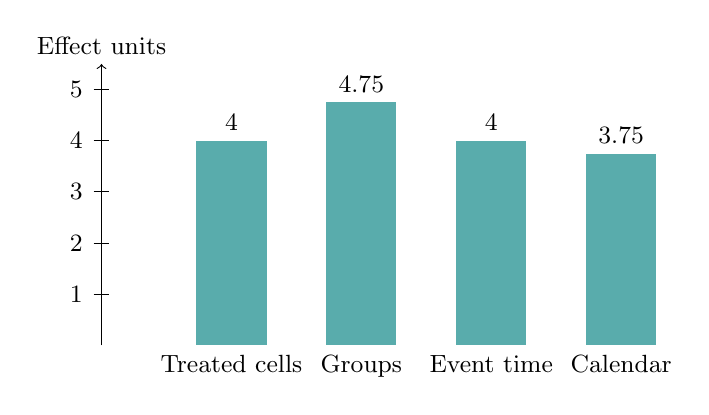
\begin{tikzpicture}[x=1.65cm,y=.65cm,every node/.style={font=\small}]
 \draw[->] (0,0)--(0,5.5) node[above]{Effect units};
 \foreach \y in {1,2,3,4,5}{\draw (-.06,\y)--(.06,\y);\node[left] at (-.07,\y){\y};}
 \foreach \x/\h in {1/4,2/4.75,3/4,4/3.75}{
  \fill[teal!65] (\x-.27,0) rectangle (\x+.27,\h);
  \node[above] at (\x,\h){\h};}
 \node[below,align=center] at (1,0){Treated\ cells};
 \node[below] at (2,0){Groups};\node[below] at (3,0){Event time};
 \node[below] at (4,0){Calendar};
\end{tikzpicture}
\caption{Different questions give different averages from the same constructed
panel. Values reproduce the two-cohort example in the R panel comparison.
They are defined averages, not empirical estimates or a ranking of packages.
\citep{exec24_panelr_contract}}
\label{reading:panel-averages}
\end{figure}

\subsection{When an implementation detail is consequential}
The selected routes in Section~\ref{rewrite:software-selection} use existing
procedures under declared targets and observation laws. A native port incurs
another implementation and validation burden; its benefit must cover that
burden. The inspected integration design develops that cost comparison.
\citep{exec16_s10_design}

These are proposal recommendations drawn from the preceding comparisons, not
claims that every integration has been executed. They also explain which
software details merit further investigation. A difference in coefficient
ordering is material when it changes reported uncertainty. A difference in a
random-number helper deserves priority only if it could change the statistical
conclusion or adoption choice. The conditional examples establish possible
failure mechanisms; they do not establish default-package defects or measured
coverage failures.~\citep{exec29_panel_inference_sources,exec29_panel_runtime_reference}

The remaining uncertainty is specific to a candidate: its supported target,
version, reuse terms or performance on the proposed study. The commercial
comparison in Section~\ref{gap29:software-followup} distinguishes those
questions from missing bank entitlements and actual prices. An unobserved
capability remains unknown. The investment decision in
Chapter~\ref{rewrite:investment-decision} compares the resulting routes.
